\documentclass{assets/utmreport}

\usepackage{booktabs,amssymb,float,graphicx,listings}

\hypersetup{hidelinks,hypertexnames=false,pdfauthor={Lucian-Adrian Gavril}}

\selectlanguage{english}

\utmlogo{assets/utm-logo.jpeg}

\institution{Technical University of Moldova}
\faculty{Faculty of Computers, Informatics, and Microelectronics}
\department{Department of Software Engineering}
\studyprogramme{Software Engineering Study Programme}
\documenttype{Laboratory report}
\reporttitle{Operating Systems Laboratory 5}
\reportsubtitle{The File System with Your Own Hands}
\student{Lucian-Adrian Gavril}{FAF-241}
\supervisor{Reițman Patricia}{univ. assist.}
\cityyear{Chișinău}{2026}

\begin{document}
\makeutmreporttitlepage
\tableofcontents
\clearpage

\begin{utmabstract}[Abstract]
This report records Linux VFS investigations described as run on Ubuntu 24.04 LTS (Linux 6.6.87.2, x86\_64) by an unprivileged UID 1000 account. Topics include namespace organization, inode metadata and directory entries, hard and symbolic links, sparse-file allocation, directory permissions, setuid, procfs, and four stretch exercises. The terminal-style figures are reconstructed illustrations, not original captures; the recorded values remain historical report observations and are not independently verified by those figures.
\utmkeywords{operating systems, linux, virtual filesystem, inodes, hard links, permissions, procfs}
\end{utmabstract}

\utmintroduction
Filesystems translate byte-oriented storage devices into hierarchical, human-navigable namespaces. Under the Unix philosophy, the abstraction extends beyond persistent media to expose device interfaces and kernel data structures through a common file interface.

Laboratory 5 explores this architecture across four core modules and four stretch problems:
\begin{utmenumerate}
\item \textbf{Filesystem Tree and Types}: Distinguishing regular files, directories, character devices, block devices, and symbolic links, alongside UsrMerge namespace organization;
\item \textbf{Inodes and Links}: Comparing directory entries with underlying inodes, hard links, dangling symbolic links, directory link count mechanics, and sparse file allocation;
\item \textbf{Permission Semantics}: Evaluating octal modes, the bitwise \texttt{umask} calculation, directory read versus execute semantics, setuid privilege elevation, and the sticky bit;
\item \textbf{Disks and Kernel Pseudo-Files}: Mapping block devices via \texttt{lsblk} and \texttt{df}, extracting hardware topology from \texttt{/proc/cpuinfo} and \texttt{/proc/meminfo}, and analyzing dynamic process resolution through \texttt{/proc/self};
\item \textbf{Advanced System Inspections}: Header magic byte parsing, setuid auditing, unlinking open file descriptors, and measuring ext4 loopback inode table sizing;
\end{utmenumerate}

\chapter{The Tree and File Types}

\section{System Root and File Type Classification}
In Unix-like systems, the first character of the \texttt{ls -l} output denotes the inode type. Inspecting \texttt{/bin}, \texttt{/dev/null}, \texttt{/etc}, \texttt{/etc/passwd}, and \texttt{/tmp} reveals five distinct filesystem abstractions:

\begin{verbatim}
$ ls -ld /etc /etc/passwd /bin /dev/null /tmp
lrwxrwxrwx   1 root root    7 Apr 22  2024 /bin -> usr/bin
crw-rw-rw-   1 root root 1, 3 Oct 12 15:33 /dev/null
drwxr-xr-x 107 root root 4096 Oct 12 15:38 /etc
-rw-r--r--   1 root root 2430 Oct 12 15:38 /etc/passwd
drwxrwxrwt  10 root root 4096 Oct 12 15:38 /tmp
\end{verbatim}

\begin{figure}[H]
\centering
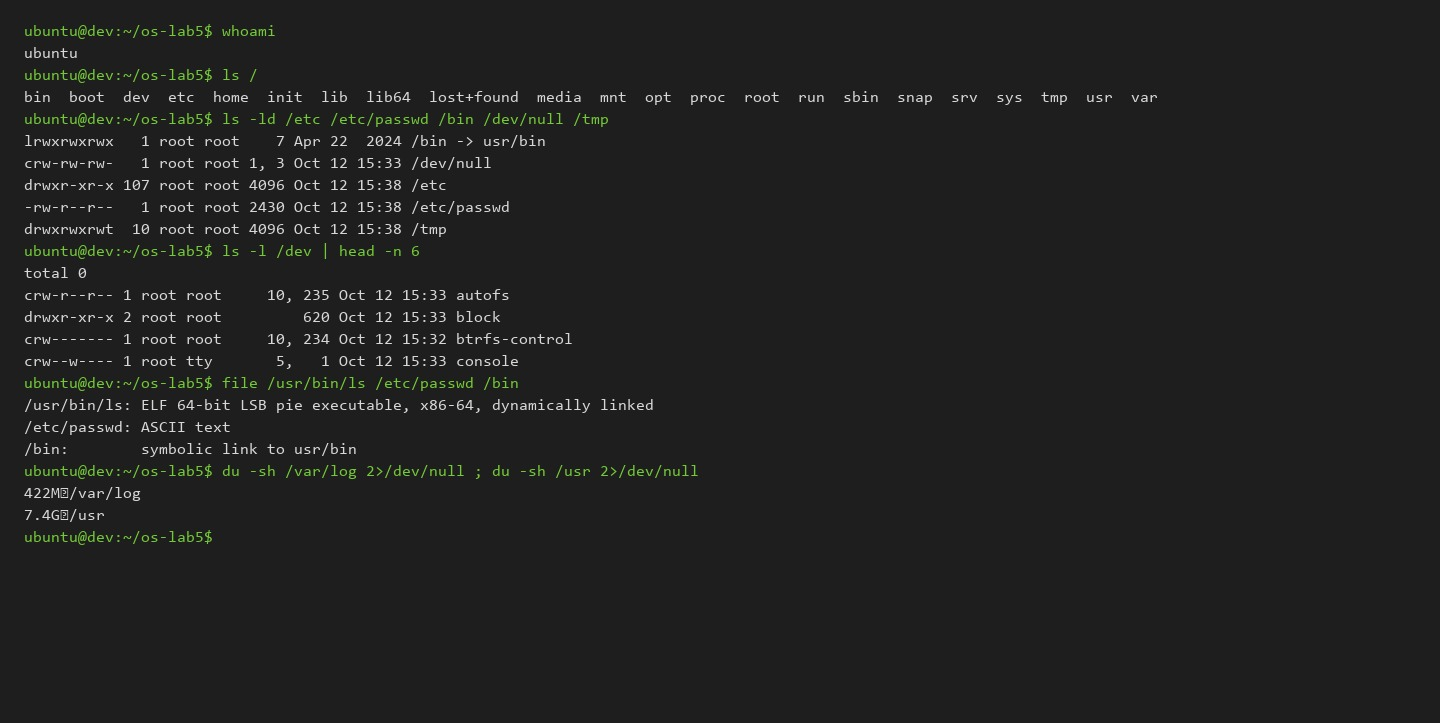
\includegraphics[width=0.92\textwidth]{assets/fig1_tree_and_types.jpg}
\caption{Reconstructed terminal illustration (not an original capture): inspecting system root, device nodes, and file types.}
\label{fig:l5_tree_types}
\end{figure}

\begin{table}[H]
\centering
\caption{File types reported in the saved 12 October run}
\begin{tabular}{lcll}
\toprule
\textbf{Path} & \textbf{Prefix} & \textbf{Filesystem Type} & \textbf{Semantic Role} \\
\midrule
\texttt{/bin} & \texttt{l} & Symbolic Link & Points to \texttt{usr/bin} (UsrMerge) \\
\texttt{/dev/null} & \texttt{c} & Character Device & Byte stream device (major 1, minor 3) \\
\texttt{/etc} & \texttt{d} & Directory & System-wide configuration table \\
\texttt{/etc/passwd} & \texttt{-} & Regular File & Plain text user database \\
\texttt{/tmp} & \texttt{d} & Directory (Sticky) & Shared workspace with mode 1777 \\
\bottomrule
\end{tabular}
\end{table}

\section{The UsrMerge Architecture}
On this system, \texttt{/bin} is a symbolic link pointing to \texttt{usr/bin}. Modern Debian and Ubuntu distributions implement UsrMerge to unify all system binaries under \texttt{/usr/bin}. This eliminates historical distinctions between essential single-user recovery binaries in \texttt{/bin} and multi-user packages in \texttt{/usr/bin}.

\section{Device Files in /dev}
Device files in \texttt{/dev} do not occupy disk data blocks; their inodes store major and minor device identifiers:
\begin{itemize}
\item \textbf{Character Device}: \texttt{/dev/null} (major 1, minor 3) streams bytes directly without intermediate caching;
\item \textbf{Block Device}: \texttt{/dev/sda} (major 8, minor 0) and \texttt{/dev/sdd} (major 8, minor 48) support random block-level transfers backed by the page cache;
\end{itemize}

\section{Filesystem Footprint: /var/log vs /usr}
Running disk utilization measurements reveals:
\begin{verbatim}
$ du -sh /var/log 2>/dev/null ; du -sh /usr 2>/dev/null
422M    /var/log
7.4G    /usr
\end{verbatim}
The \texttt{/usr} hierarchy occupies 7.4 GB, which is roughly 7.0 GB larger ($\approx 17.5 \times$) than \texttt{/var/log} (422 MB). This disparity is expected because \texttt{/usr} houses shared libraries, system utilities, compilers, headers, and documentation, whereas \texttt{/var/log} only stores log text.

\chapter{Inodes, Links, and Space Allocation}

\section{Inode Metadata and Hard Links}
A file's human-readable name is not stored within its inode. It exists solely as an entry in a parent directory mapping a string to an inode number. Figure \ref{fig:l5_links_concept} summarizes the relationship; its open-file-table layer is omitted.

\begin{figure}[H]
\centering
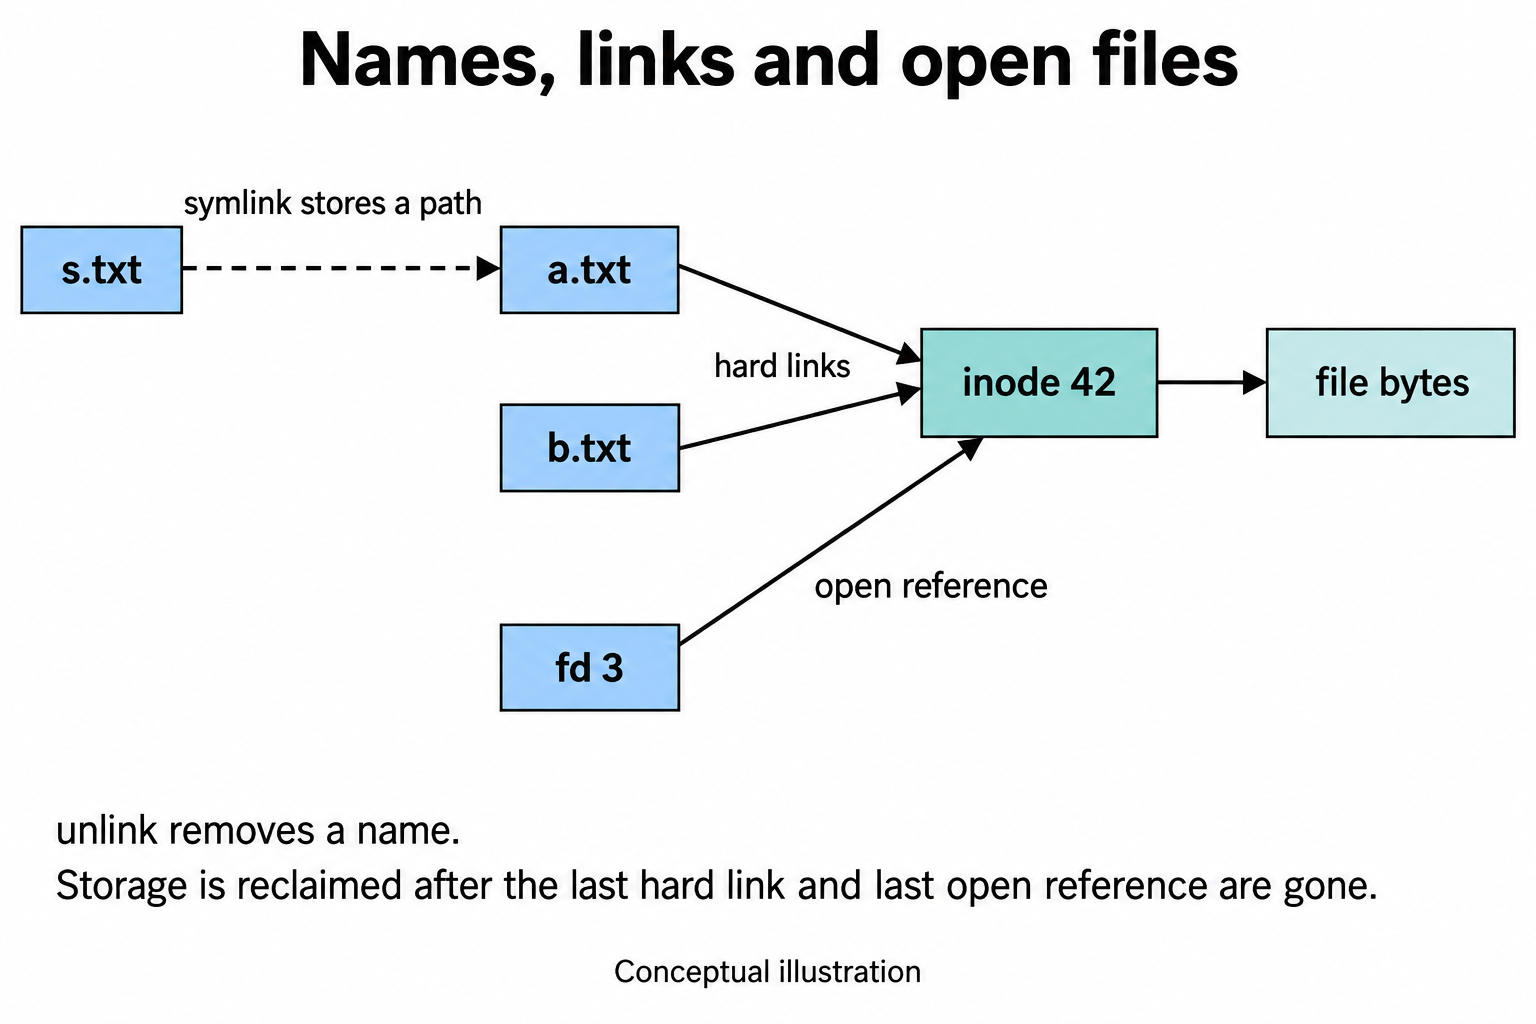
\includegraphics[width=0.88\textwidth]{assets/concept-filesystem-links.png}
\caption{Conceptual diagram of names, inodes, and links; the open-file-table layer is omitted. Generated illustration, not execution evidence.}
\label{fig:l5_links_concept}
\end{figure}

\begin{verbatim}
$ echo hello > notes.txt
$ stat notes.txt
  File: notes.txt
  Size: 6           Blocks: 8          IO Block: 4096   regular file
Device: 8,48    Inode: 18829       Links: 1
\end{verbatim}

Creating a hard link creates a second directory entry referencing the identical inode:
\begin{verbatim}
$ ln notes.txt hard.txt
$ ls -li notes.txt hard.txt
18829 -rw-r--r-- 2 ubuntu ubuntu 6 Oct 12 15:39 hard.txt
18829 -rw-r--r-- 2 ubuntu ubuntu 6 Oct 12 15:39 notes.txt
$ rm notes.txt
$ cat hard.txt
hello
\end{verbatim}

\begin{figure}[H]
\centering
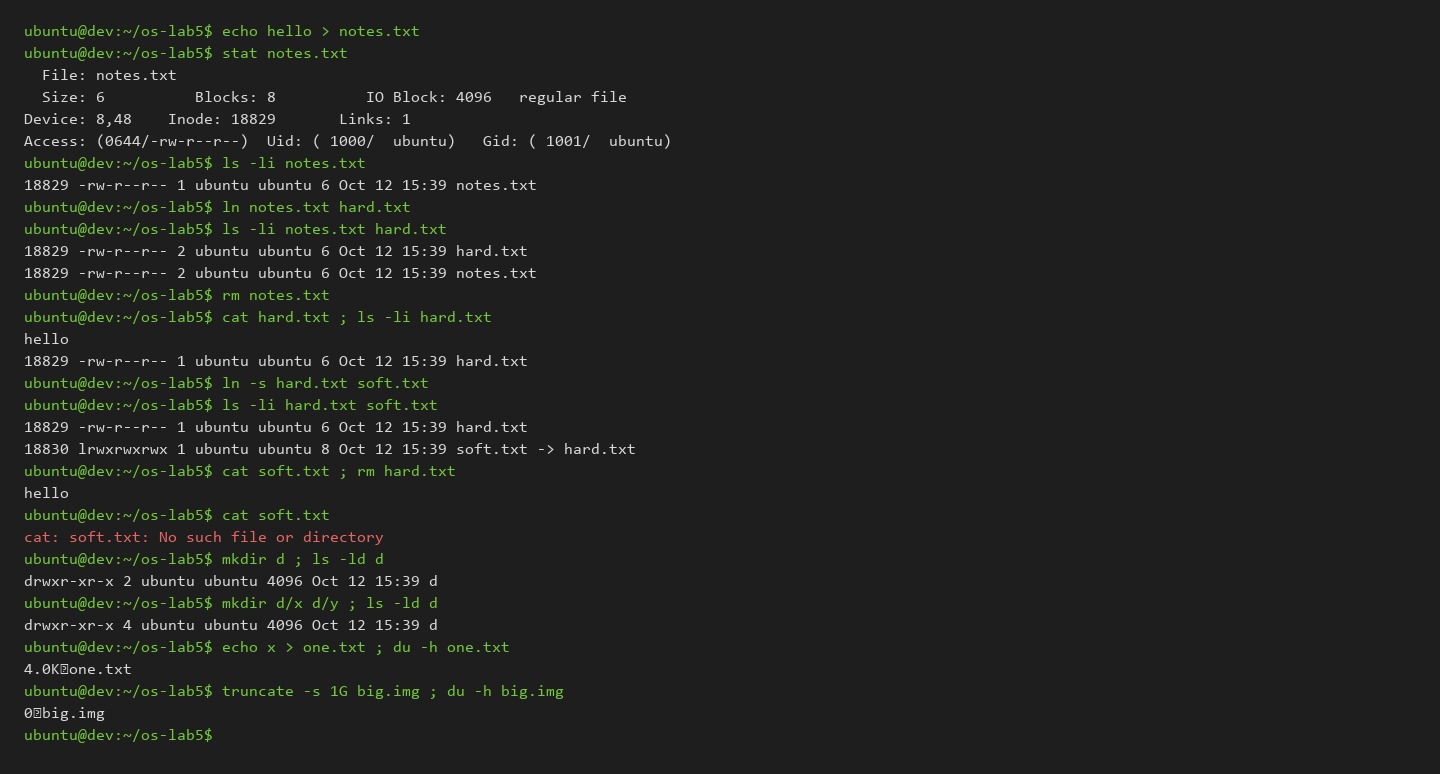
\includegraphics[width=0.92\textwidth]{assets/fig2_inodes_and_links.jpg}
\caption{Reconstructed terminal illustration (not an original capture): inode inspection, hard links, dangling symlinks, and sparse files.}
\label{fig:l5_inodes_links}
\end{figure}

The \texttt{rm} utility invokes \texttt{unlink()}, removing the name \texttt{notes.txt} from the directory and decrementing \texttt{i\_nlink} from 2 to 1. Because \texttt{hard.txt} still points to inode 18829 and the link counter is positive, data blocks remain on disk.

\section{Symbolic Link Mechanics}
Unlike hard links, symbolic links are distinct inodes storing the path string of their target:
\begin{verbatim}
$ ln -s hard.txt soft.txt
$ ls -li hard.txt soft.txt
18829 -rw-r--r-- 1 ubuntu ubuntu 6 Oct 12 15:39 hard.txt
18830 lrwxrwxrwx 1 ubuntu ubuntu 8 Oct 12 15:39 soft.txt -> hard.txt
$ rm hard.txt
$ cat soft.txt
cat: soft.txt: No such file or directory
\end{verbatim}
When \texttt{hard.txt} is removed, \texttt{soft.txt} becomes a dangling link. Opening it fails with \texttt{ENOENT}. The length of \texttt{soft.txt} is exactly 8 bytes because the path string \texttt{"hard.txt"} contains 8 characters.

\section{Directory Link Count Arithmetic}
Directories have fixed link counting rules:
\begin{verbatim}
$ mkdir d ; ls -ld d
drwxr-xr-x 2 ubuntu ubuntu 4096 Oct 12 15:39 d
$ mkdir d/x d/y ; ls -ld d
drwxr-xr-x 4 ubuntu ubuntu 4096 Oct 12 15:39 d
\end{verbatim}
A new directory starts with 2 links: the parent entry \texttt{d} and the self-referencing entry \texttt{d/.}. When child directories \texttt{d/x} and \texttt{d/y} are created, each child contains a \texttt{..} entry pointing back to \texttt{d}, raising the link count to 4.

\section{Logical Size versus Physical Allocation}
File systems allocate storage in discrete blocks (4096 bytes in ext4):
\begin{verbatim}
$ echo x > one.txt ; ls -l one.txt ; du -h one.txt
-rw-r--r-- 1 ubuntu ubuntu 2 Oct 12 15:39 one.txt
4.0K    one.txt

$ truncate -s 1G big.img ; ls -lh big.img ; du -h big.img
-rw-r--r-- 1 ubuntu ubuntu 1.0G Oct 12 15:39 big.img
0       big.img
\end{verbatim}
A 2-byte file requires one full 4 KiB filesystem block. Conversely, \texttt{truncate} creates a sparse file: it updates \texttt{i\_size} in the inode metadata to 1 GiB without writing data blocks, resulting in 0 physical blocks allocated.

\chapter{Permissions and Access Control}

\section{Octal Modes and Evaluation Semantics}
File permissions represent three 3-bit masks for User, Group, and Others:
\begin{itemize}
\item \texttt{600} (\texttt{rw-------}): Private SSH keys (\texttt{\~{}/.ssh/id\_rsa});
\item \texttt{644} (\texttt{rw-r--r--}): Web assets, documentation, \texttt{/etc/passwd};
\item \texttt{755} (\texttt{rwxr-xr-x}): Executables (\texttt{/bin/ls}) and public directories;
\item \texttt{700} (\texttt{rwx------}): Private directories (\texttt{\~{}/.ssh});
\end{itemize}

When setting \texttt{chmod 000 s.txt}, reading fails even for the file's owner:
\begin{verbatim}
$ chmod 000 s.txt ; cat s.txt
cat: s.txt: Permission denied
\end{verbatim}
The kernel checks whether \texttt{current\_euid == inode->i\_uid}. Since it matches, only owner bits are evaluated. Because owner bits are \texttt{0}, access is denied immediately. Ownership provides the authority to change mode bits with \texttt{chmod()}, not an automatic read bypass.

\begin{figure}[H]
\centering
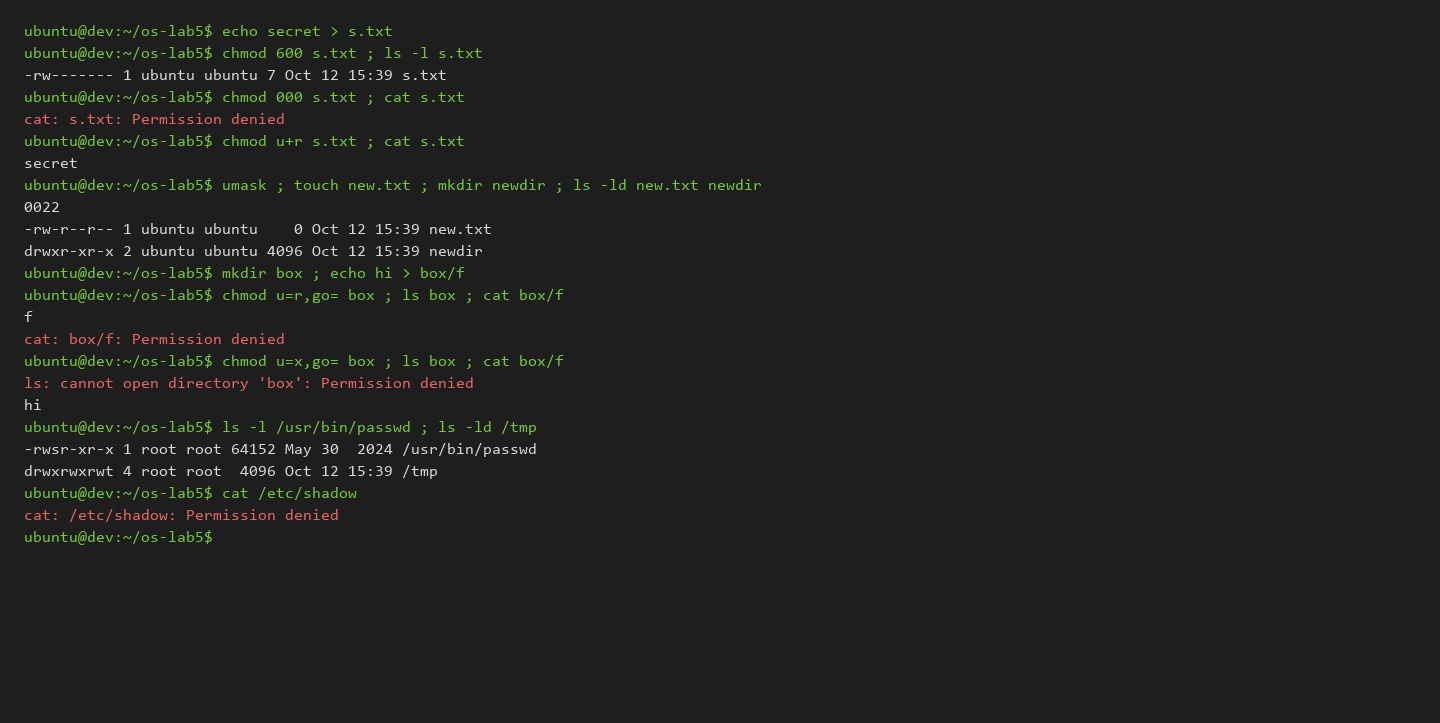
\includegraphics[width=0.92\textwidth]{assets/fig3_permissions.jpg}
\caption{Reconstructed terminal illustration (not an original capture): permission evaluation, umask verification, and directory traversal.}
\label{fig:l5_permissions}
\end{figure}

\section{The umask Calculation}
The observed \texttt{umask} is \texttt{0022}:
\begin{verbatim}
$ umask ; touch new.txt ; mkdir newdir ; ls -ld new.txt newdir
0022
-rw-r--r-- 1 ubuntu ubuntu    0 Oct 12 15:39 new.txt
drwxr-xr-x 2 ubuntu ubuntu 4096 Oct 12 15:39 newdir
\end{verbatim}
Files start from base mode \texttt{0666}: $0666 \ \& \ \sim 0022 = 0644$ (\texttt{rw-r--r--}). Directories start from base mode \texttt{0777}: $0777 \ \& \ \sim 0022 = 0755$ (\texttt{rwxr-xr-x}).

\section{Directory Read versus Execute Permissions}
The \texttt{box} directory experiment demonstrates the separation between listing and traversing:
\begin{verbatim}
# Read-only directory
$ chmod u=r,go= box ; ls box ; cat box/f
f
cat: box/f: Permission denied

# Execute-only directory
$ chmod u=x,go= box ; ls box ; cat box/f
ls: cannot open directory 'box': Permission denied
hi
\end{verbatim}
Read permission (\texttt{r}) allows reading the directory table, permitting \texttt{ls} to show the name \texttt{f}. However, traversing into the directory requires execute permission (\texttt{x}). Without \texttt{x}, path resolution fails. With execute-only permission (\texttt{x}), directory listing fails, but accessing known files directly succeeds.

\section{Setuid and the Sticky Bit}
\begin{verbatim}
$ ls -l /usr/bin/passwd ; ls -ld /tmp
-rwsr-xr-x 1 root root 64152 May 30  2024 /usr/bin/passwd
drwxrwxrwt 4 root root  4096 Oct 12 15:39 /tmp
\end{verbatim}
The \texttt{s} in \texttt{/usr/bin/passwd} denotes setuid. When executed, the process assumes the effective UID of the file owner (\texttt{root}). This allows \texttt{passwd} to modify \texttt{/etc/shadow}, which normal users cannot write to. The \texttt{t} in \texttt{/tmp} represents the sticky bit: in a shared world-writable directory, users may only delete or rename files they own.

\chapter{Disks, Topology, and Kernel Pseudo-Files}

\section{Disk Layout and Root Mount}
\begin{verbatim}
$ lsblk
NAME MAJ:MIN RM   SIZE RO TYPE MOUNTPOINTS
sdc    8:32   0     5G  0 disk [SWAP]
sdd    8:48   0     1T  0 disk /

$ df -h
Filesystem      Size  Used Avail Use% Mounted on
/dev/sdd       1007G  4.2G  952G   1% /

$ mount | grep " / "
/dev/sdd on / type ext4 (rw,relatime,discard,errors=remount-ro,data=ordered)
\end{verbatim}

\begin{figure}[H]
\centering
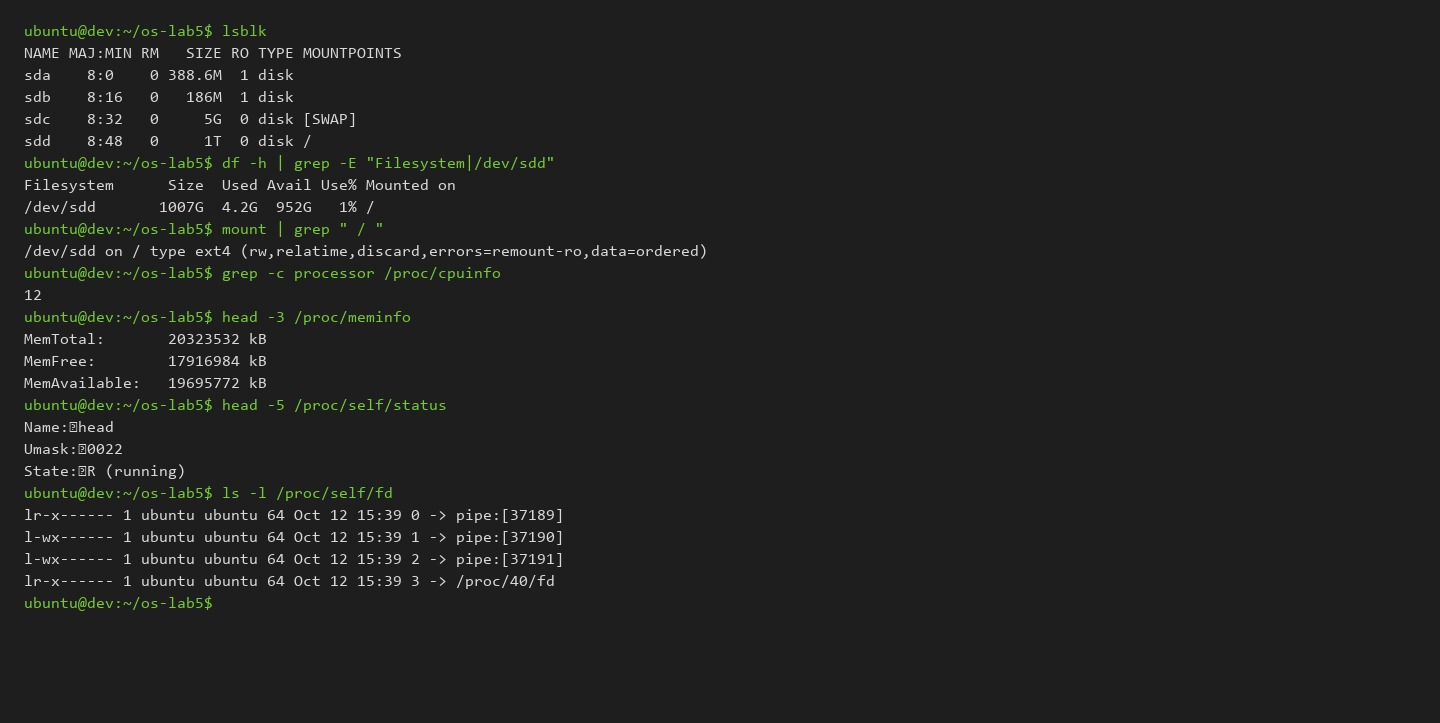
\includegraphics[width=0.92\textwidth]{assets/fig4_disks_and_proc.jpg}
\caption{Reconstructed terminal illustration (not an original capture): disk topology, mount attributes, and procfs inspection.}
\label{fig:l5_disks_proc}
\end{figure}

The root filesystem resides on \texttt{/dev/sdd}, a 1 TB virtual SCSI disk formatted with ext4. It has 4.2 GB allocated out of 1007 GB (1\% utilization). Swap is allocated on \texttt{/dev/sdc} (5 GB).

\section{Hardware Introspection via /proc}
\begin{verbatim}
$ grep -c processor /proc/cpuinfo
12
$ head -3 /proc/meminfo
MemTotal:       20323532 kB
MemFree:        17916984 kB
MemAvailable:   19695772 kB
\end{verbatim}
The host exposes 12 logical CPU cores and 20,323,532 kB ($\approx 19.38$ GiB) of total RAM.

\section{Self Process Resolution in /proc/self}
\begin{verbatim}
$ head -5 /proc/self/status
Name:   head
Umask:  0022
State:  R (running)
\end{verbatim}
The reported process name is \texttt{head}. In Linux, \texttt{/proc/self} is a dynamic symlink that resolves to the PID of the accessing process. Because \texttt{head} opens \texttt{/proc/self/status}, the kernel reports the status of \texttt{head}.

\chapter{Stretch Experiments}

\begin{figure}[H]
\centering
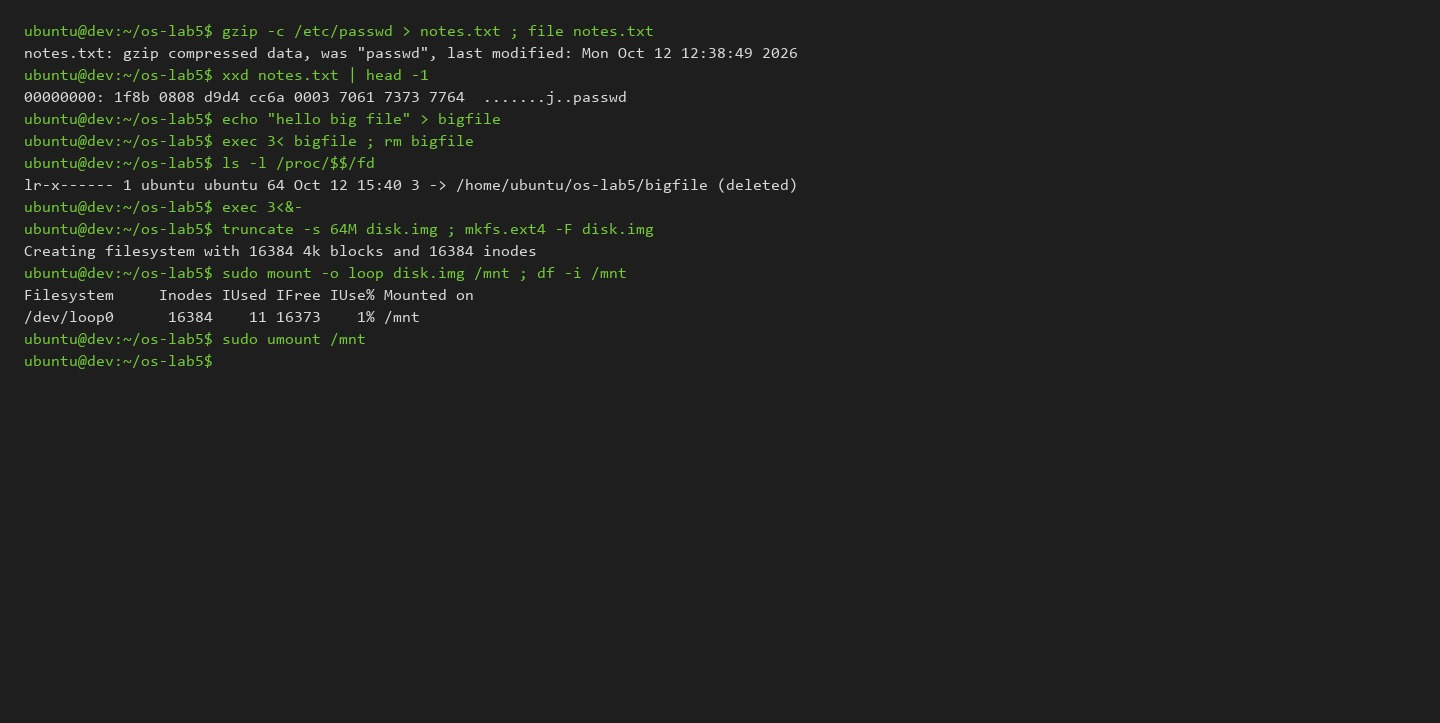
\includegraphics[width=0.92\textwidth]{assets/fig5_stretch.jpg}
\caption{Reconstructed terminal illustration (not an original capture): magic bytes, unlinking open file descriptors, and ext4 loopback mount.}
\label{fig:l5_stretch}
\end{figure}

\section{(a) Magic Number Header Inspection}
\begin{verbatim}
$ gzip -c /etc/passwd > notes.txt
$ xxd notes.txt | head -1
00000000: 1f8b 0808 d9d4 cc6a 0003 7061 7373 7764  .......j..passwd
\end{verbatim}
The first two bytes, \texttt{0x1f 0x8b}, are the gzip magic number per RFC 1952. The \texttt{file} utility uses these bytes to identify the file type regardless of filename extension.

\section{(b) Setuid Binary Audit}
A system scan reveals essential setuid binaries:
\begin{verbatim}
/usr/bin/passwd, /usr/bin/su, /usr/bin/sudo, /usr/bin/mount, /usr/bin/umount,
/usr/lib/polkit-1/polkit-agent-helper-1, /usr/lib/openssh/ssh-keysign
\end{verbatim}

\section{(c) Unlinking an Open File Descriptor}
\begin{verbatim}
$ exec 3< bigfile ; rm bigfile
$ ls -l /proc/$$/fd
lr-x------ 1 ubuntu ubuntu 64 Oct 12 15:40 3 -> /home/ubuntu/os-lab5/bigfile (deleted)
$ exec 3<&-
\end{verbatim}
The link target indicates \texttt{(deleted)}. The directory entry is removed, but the inode and data blocks remain allocated until the last open descriptor is closed via \texttt{exec 3<\&-}.

\section{(d) Loopback ext4 Inode Allocation}
\begin{verbatim}
$ truncate -s 64M disk.img ; mkfs.ext4 -F disk.img
Creating filesystem with 16384 4k blocks and 16384 inodes
$ sudo mount -o loop disk.img /mnt ; df -i /mnt
Filesystem     Inodes IUsed IFree IUse% Mounted on
/dev/loop0      16384    11 16373    1% /mnt
\end{verbatim}
Formatting a 64 MiB disk image created exactly 16,384 inodes (one inode per 4 KiB block).

\utmconclusions
The saved command transcript and source analysis illustrate the separation between names and inode metadata: unlinking a name does not free data blocks while hard links or open descriptors remain, sparse files separate logical size from allocation, and directory read and execute permissions control enumeration and traversal differently. The terminal-style figures are reconstructed illustrations rather than original captures; the reported values remain historical and unverified.

\appendix
\chapter{Focused WSL Demonstration, 23 October 2026}
\section{Environment and scope}
The captured execution record is \texttt{execution-2026-10-23.txt}. It records one bounded Ubuntu 24.04.4 WSL2 user-space run on the WSL2 Linux 6.18.33.2 kernel. The tests ran in an ext4 temporary directory under \texttt{/tmp} using Bash 5.2.21, GNU coreutils 9.4, and Python 3.12.3. They covered hard links, symbolic-link metadata, reading through an open descriptor after unlink, and sparse allocation. No filesystem image was mounted, no special permission bit was changed, and the other historical report experiments were not repeated.

\section{Selected captured output}
\begin{verbatim}
name=target.txt type=regular file inode=105838 links=2 size=10 bytes
name=hardlink.txt type=regular file inode=105838 links=2 size=10 bytes
link=symlink.txt type=symbolic link inode=105839
referent=symlink.txt type=regular file inode=105838 links=2
hardlink after original name removed: hardlink.txt inode=105838 links=1 size=10 bytes
name_exists=False fd_links=0 bytes_read=28 data='still readable after unlink'
sparse=sparse.bin logical_bytes=1048576 allocated_512_byte_blocks=0 block_size=512
1048576 sparse.bin
\end{verbatim}

The two hard-link names initially refer to inode 105838. Removing \texttt{target.txt} leaves \texttt{hardlink.txt} with one link. The open descriptor remains readable after unlink even though its inode reports zero directory links. In this ext4 run, the sparse file has a logical size of 1,048,576 bytes and zero allocated 512-byte accounting blocks. The 512-byte unit is the allocation-count accounting unit, not the ext4 filesystem block size; du reported zero allocated bytes. These fresh results cover only the listed operations; the older terminal panels and other recorded measurements remain historical report material.
\end{document}
